%!TEX root = ../main.tex
\chapter{Basics}
In order to carry out the analysis and the intended concept, knowledge of the programs used as well as the environment is necessary first. Therefore, the most important parts of the figure 3.1 are shown in the following sections.

\begin{figure}[!ht]
	\centering
		%[natürliche Breite in Pixeln, natürliche Höhe in Pixeln, Abhängigkeit von der Textbreite]
		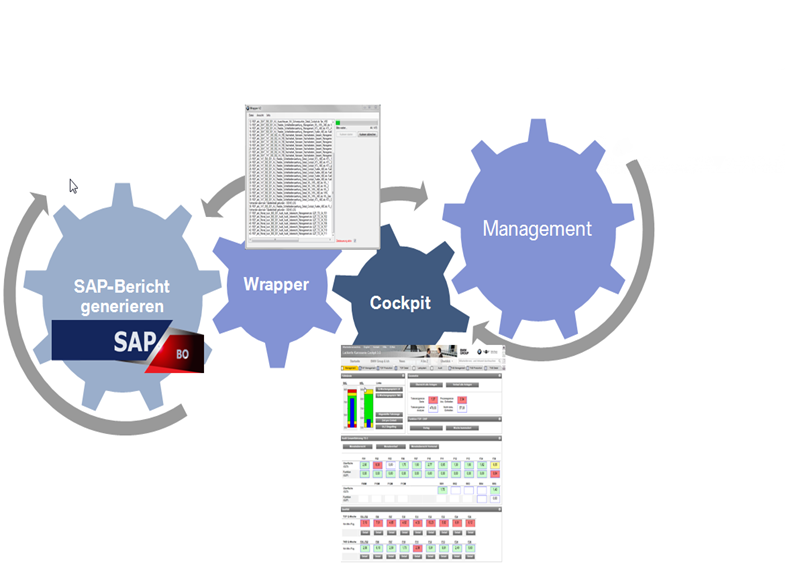
\includegraphics[width=845pt, height=258pt, width=1.0\textwidth]{images/3_1.png}
	\caption[Interaction between SAP BO, Wrapper, and Cockpit]{Interaction between SAP Bo, Wrapper, and Cockpit\footnotemark} 
	\label{fig:Interaction between SAP BO, Wrapper, Cockpit}

\end{figure}
\footnotetext{(BMW AG, Department presentation-TD300)}
\section{Reporting creation environment }
In the reporting environment, SAP BO plays the main role. From the data modeling to report creation all necessary works for reporting are done by SAP BO tools. The reports generated from SAP BO tools further used by wrapper and cockpit.
\subsection{Information Design Tool (IDT)}
Information Design tool (IDT) is a part of SAP BO tools. This tool is using for extracting, defining  and manipulating data from different databases in order to create semantic layer for different reporting tools. Data modeling, data restriction, data optimization, data analysis and  various calculations over dimension or measures are performing by this tool. The final output from this tools is a semantic layer for business users, which is called as universe. The universe further used by different reporting tools for report creation.
\subsection{Web Intelligence (Webi)}
Webi provide users an easy-to-use, interactive and flexible user interface for creating and analyzing reports over the intranet. Web intelligence can be used by employees via their browser. After authentication, the reports can be used interactively, depending on the user role, or can be created or edited using a report editor. Webi allows to create both management reports and detail report, which can be used to analyze various data. After the universe creation this tool is used for generating different kinds of report based on available objects in the underlying universe.There are different kinds of report generating from this department such as Ad-hoc report, detail report, interactive report etc. 
\subsection{Central Management Console (CMC)}
The central management Console (CMC) is the main interface to perform the administrative tasks in SAP BO Objects. This tools helps to organize servers, users, folders, security, as well as report scheduling and observing the performance of the overall system.
\section{Wrapper}
The Wrapper is an interface tool between SAP BO and Cockpit, which developed by this department TD-300. This tool extract the KPI values from the report and save those values with different meaningful colors in image format. The images produce from Wrapper are using in the Cockpit to show the KPIs to the top level management. This tool can extract the required data from different file formats. \newpage

\section{Cockpit}
The Cockpit is a very end user web interface tool for report presentation. Cockpit contains KPIs and associate detail report for different department in a precise way. This tools serves lot of useful features for the end users. KPIs showing in different colors to understand the production condition at a glance. At this moment, Cockpit showing KPIs on daily basis, and monthly basic with detail report and providing direct web intelligence report links for interactive data analysis. This tool also developed by this department, TD-300.\\

\begin{figure}[!ht]
	\centering
		%[natürliche Breite in Pixeln, natürliche Höhe in Pixeln, Abhängigkeit von der Textbreite]
		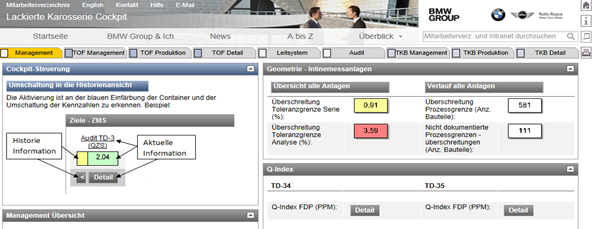
\includegraphics[width=598pt, height=229pt, width=1.0\textwidth]{images/cockpit.png}
	\caption[Cockpit]{Cockpit\footnotemark} 
	\label{fig:Cockpit}

\end{figure}
\footnotetext{(BMW AG, Department presentation-TD300)}

\newpage

\section{IPS-Q (International Production System Quality Assurance)}
IPS-Q databases stores all the production data. There are different types of IPS-Q databases. The most important database is productive database which contains all the current production data and copy to the IPS-Q evaluation database. When data is older than 65 days then data copy to the history database and remove from evaluation database. When data is older than 3 years then data copy to central historical database. The reports are generation from all those databases for covering different purpose. \\

\begin{figure}[!ht]
	\centering
		%[natürliche Breite in Pixeln, natürliche Höhe in Pixeln, Abhängigkeit von der Textbreite]
		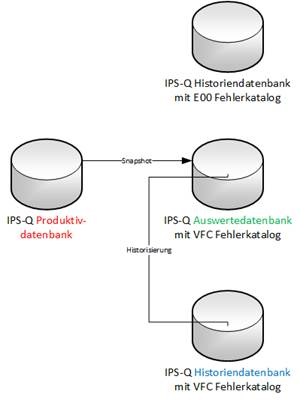
\includegraphics[width=300pt, height=400pt, width=1.0\textwidth]{images/3_2_IPSQ.jpg}
	\caption[IPS-Q Databases]{IPS-Q Databases\footnotemark} 
	\label{fig:IPS-Q Databases}

\end{figure}
\footnotetext{(BMW AG, Department presentation-TD300)}
